\section{Sonderfälle}
\subsection{Einführung}
Beim Lösen der linearen Optimierungsprobleme können verschiedene Sonderfälle auftreten. Hierbei kann es zu unendlich vielen oder keiner optimalen oder zulässigen Lösung kommen.
Es gibt vier verschiedene Sonderfälle: die unbeschränkte Lösung, mehrere optimale Lösungen, keine zulässige Lösung und die degenerierte Lösung, welche nachfolgend genauer beschrieben werden.\\\\
\textbf{Unbeschränkte Lösung:}\\\\
Der Fall der unbeschränkten Lösung tritt auf, wenn es zur Wahl der Pivotzeile kommt. Wie bereits zuvor beschrieben, wird diese ermittelt, indem die Werte aus der Pivotspalte durch die dazugehörigen Werte aus der rechten Spalte dividiert werden. Jedoch müssen die Werte der Pivotspalte hierfür größer Null sein. Ist dies nicht gegeben, kann keine geeignete Pivotzeile bestimmt werden und es gibt somit keine optimale Lösung des Problems.
\\\\
\textbf{Beispiel:}\\\\
Zielfunktion: max Z = 10 * $x_1$+5 * $x_2$\\
Nebenbedingungen:\\\begin{math}
6*x_1-12*x_2 <= 60\\
-2*x_1+2*x_2 <= 50\\
-3*x_1 +1*x_2 <= 15\\\end{math}
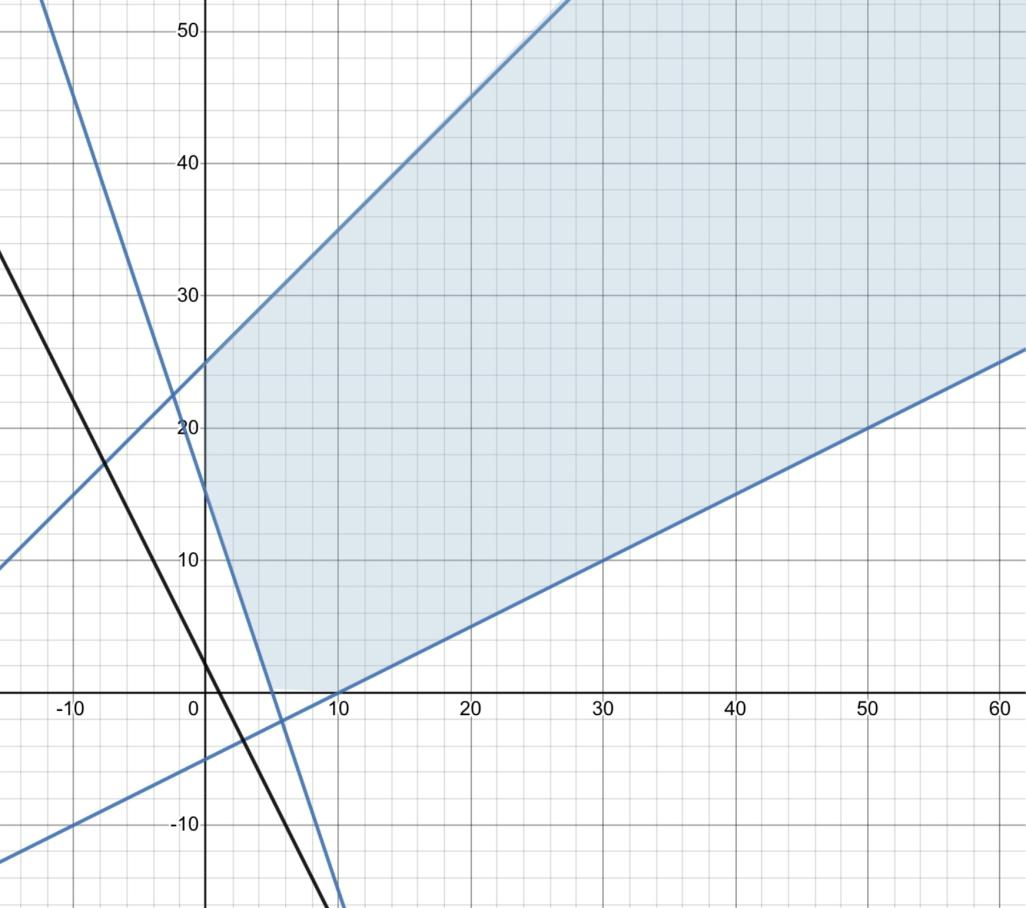
\includegraphics[width=5cm,right]{images/IMG_unbeschrankte_Losung.jpeg}
\\\\
Nichtnegativitätsbedingung:
\begin{math}1 <= 0, x_2 <= 0 \end{math}\\
\begin{table}[h]
\begin{tabular}{|l|l|l|l|l|l|l|}
\hline
\rowcolor[HTML]{C0C0C0} 
Zeile                     & $x_1$                         & $x_2$                          & $s_1$                        & $s_2$                        & $s_3$                        & RS \\ \hline
\cellcolor[HTML]{C0C0C0}1 & \cellcolor[HTML]{96FFFB}6  & \cellcolor[HTML]{FFFFFF}-12 & \cellcolor[HTML]{FFFFFF}1 & \cellcolor[HTML]{FFFFFF}0 & \cellcolor[HTML]{FFFFFF}0 & 60 \\ \hline
\cellcolor[HTML]{C0C0C0}2 & \cellcolor[HTML]{FFFFFF}-2 & \cellcolor[HTML]{FFFFFF}2   & \cellcolor[HTML]{FFFFFF}0 & \cellcolor[HTML]{FFFFFF}1 & \cellcolor[HTML]{FFFFFF}0 & 50 \\ \hline
\cellcolor[HTML]{C0C0C0}3 & \cellcolor[HTML]{FFFFFF}-3 & \cellcolor[HTML]{FFFFFF}1   & \cellcolor[HTML]{FFFFFF}0 & \cellcolor[HTML]{FFFFFF}0 & \cellcolor[HTML]{FFFFFF}1 & 15 \\ \hline
\cellcolor[HTML]{C0C0C0}Z & -10                        & -5                          & 0                         & 0                         & 0                         & 0  \\ \hline
\end{tabular}
\end{table}
\\
\begin{table}[!ht]
\begin{tabular}{|l|l|l|l|l|l|l|l|}
\hline
\rowcolor[HTML]{C0C0C0} 
Zeile                     & $x_1$                        & $x_2$                                  & $s_1$                          & $s_2$                        & $s_3$                        & RS  & Rechnung                \\ \hline
\cellcolor[HTML]{C0C0C0}1 & \cellcolor[HTML]{FFFFFF}1 & \cellcolor[HTML]{FFFFFF}\textbf{-2} & \cellcolor[HTML]{FFFFFF}1/6 & \cellcolor[HTML]{FFFFFF}0 & \cellcolor[HTML]{FFFFFF}0 & 10  & (wurde durch 6 geteilt) \\ \hline
\cellcolor[HTML]{C0C0C0}2 & \cellcolor[HTML]{FFFFFF}0 & \cellcolor[HTML]{FFFFFF}\textbf{-2} & \cellcolor[HTML]{FFFFFF}1/3 & \cellcolor[HTML]{FFFFFF}1 & \cellcolor[HTML]{FFFFFF}0 & 70  & +2*(Zeile 1)            \\ \hline
\cellcolor[HTML]{C0C0C0}3 & \cellcolor[HTML]{FFFFFF}0 & \cellcolor[HTML]{FFFFFF}\textbf{-5} & \cellcolor[HTML]{FFFFFF}1/2 & \cellcolor[HTML]{FFFFFF}0 & \cellcolor[HTML]{FFFFFF}1 & 45  & +3*(Zeile 1)            \\ \hline
\cellcolor[HTML]{C0C0C0}Z & 0                         & \textbf{-25}                        & 5/3                         & 0                         & 0                         & 100 & +10*(Zeile 1)           \\ \hline
\end{tabular}
\end{table}
\\
In diesem Beispiel kann der erste Iterationsschritt noch normal ausgeführt werden. Bei dem zweiten Iterationsschritt stößt man jedoch auf ausschließlich negative Werte in der Pivotspalte - somit kann keine optimale Lösung ermittelt werden.
\\\\\\
\textbf{Mehrere optimale Lösungen (unendlich viele Lösungen):}\\
In diesem Fall kann es mehrere optimale Lösungen des Optimierungsproblems geben. Dies wird im Optimaltableau erkennbar, wenn mindestens ein Wert in der Zeile der Zielfunktion einer Nichtbasisvariablen den Wert Null hat. Nimmt man diese mit in die Basis auf, ergibt sich eine weitere optimale Lösung.
\\\\
\textbf{Beispiel:}\\
Zielfunktion: max \begin{math}Z = 3*x_1+3*x_2\end{math}\\
Nebenbedingungen:\\
\begin{math}
3*x_1+3*x_2 <= 60\\
-1*x_1+1*x_2 <= 15\\
1*x_1 <= 15\\
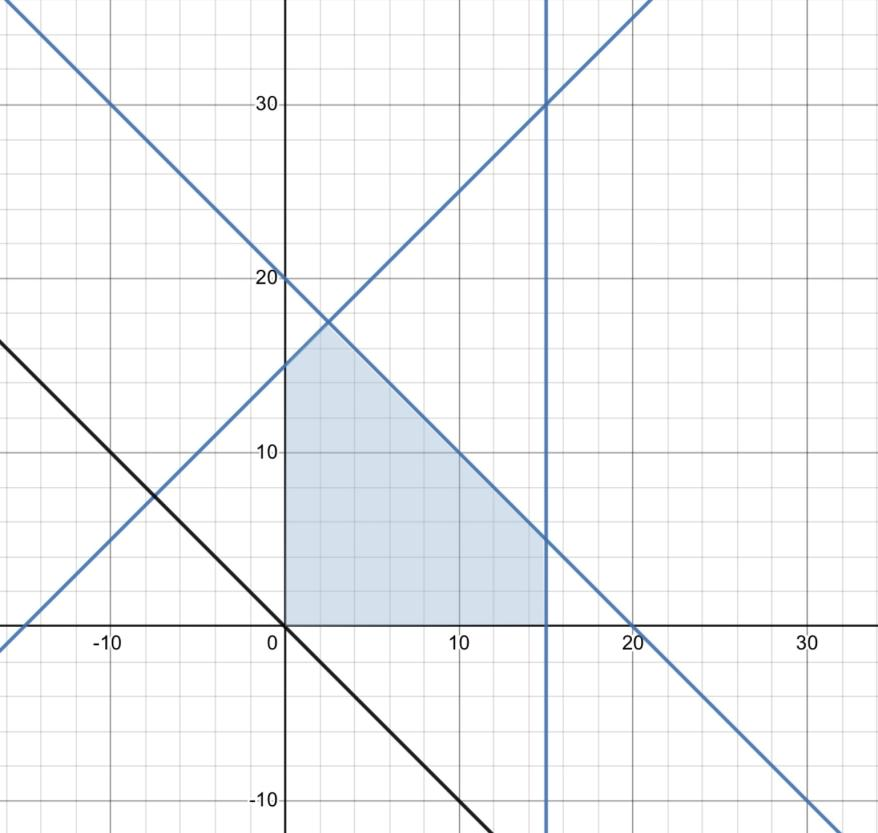
\includegraphics[width = 5cm, right]{images/IMG_unendlich_viele_Losungen.jpeg}
\end{math}\\
Nichtnegativitätsbedingung:\\
\begin{math}
x_1 >= 0, x_2 >= 0
\end{math}
\\
\begin{table}[!ht]
\begin{tabular}{|l|l|l|l|l|l|l|}
\hline
\rowcolor[HTML]{C0C0C0} 
Zeile                     & $x_1$                         & $x_2$                        & $s_1$                        & $s_2$                        & $s_3$                        & RS \\ \hline
\cellcolor[HTML]{C0C0C0}1 & \cellcolor[HTML]{FFFFFF}3  & \cellcolor[HTML]{FFFFFF}3 & \cellcolor[HTML]{FFFFFF}1 & \cellcolor[HTML]{FFFFFF}0 & \cellcolor[HTML]{FFFFFF}0 & 60 \\ \hline
\cellcolor[HTML]{C0C0C0}2 & \cellcolor[HTML]{FFFFFF}-1 & \cellcolor[HTML]{FFFFFF}1 & \cellcolor[HTML]{FFFFFF}0 & \cellcolor[HTML]{FFFFFF}1 & \cellcolor[HTML]{FFFFFF}0 & 15 \\ \hline
\cellcolor[HTML]{C0C0C0}3 & \cellcolor[HTML]{DAE8FC}1  & \cellcolor[HTML]{FFFFFF}0 & \cellcolor[HTML]{FFFFFF}0 & \cellcolor[HTML]{FFFFFF}0 & \cellcolor[HTML]{FFFFFF}1 & 15 \\ \hline
\cellcolor[HTML]{C0C0C0}Z & -3                         & -3                        & 0                         & 0                         & 0                         & 0  \\ \hline
\end{tabular}
\end{table}
\\
\begin{table}[!ht]
\begin{tabular}{|l|l|l|l|l|l|l|l|}
\hline
\rowcolor[HTML]{C0C0C0} 
Zeile                     & $x_1$                        & $x_2$                        & $s_1$                        & $s_2$                        & $s_3$                         & RS & Rechnung     \\ \hline
\cellcolor[HTML]{C0C0C0}1 & \cellcolor[HTML]{FFFFFF}0 & \cellcolor[HTML]{CBCEFB}3 & \cellcolor[HTML]{FFFFFF}1 & \cellcolor[HTML]{FFFFFF}0 & \cellcolor[HTML]{FFFFFF}-3 & 15 & -3*(Zeile 3) \\ \hline
\cellcolor[HTML]{C0C0C0}2 & \cellcolor[HTML]{FFFFFF}0 & \cellcolor[HTML]{FFFFFF}1 & \cellcolor[HTML]{FFFFFF}0 & \cellcolor[HTML]{FFFFFF}1 & \cellcolor[HTML]{FFFFFF}1  & 30 & +(Zeile 3)   \\ \hline
\cellcolor[HTML]{C0C0C0}3 & \cellcolor[HTML]{FFFFFF}1 & \cellcolor[HTML]{FFFFFF}0 & \cellcolor[HTML]{FFFFFF}0 & \cellcolor[HTML]{FFFFFF}0 & \cellcolor[HTML]{FFFFFF}1  & 15 &              \\ \hline
\cellcolor[HTML]{C0C0C0}Z & 0                         & -3                        & 0                         & 0                         & 3                          & 45 & +3*(Zeile 3) \\ \hline
\end{tabular}
\end{table}
\\
\begin{table}[!ht]
\begin{tabular}{|l|l|l|l|l|l|l|l|}
\hline
\rowcolor[HTML]{C0C0C0} 
Zeile                     & $x_1$ & $x_2$ & $s_1$   & $s_2$ & $s_3$ & RS & Rechnung                \\ \hline
\rowcolor[HTML]{FFFFFF} 
\cellcolor[HTML]{C0C0C0}1 & 0  & 1  & 1/3  & 0  & -1 & 5  & (wurde durch 3 geteilt) \\ \hline
\rowcolor[HTML]{FFFFFF} 
\cellcolor[HTML]{C0C0C0}2 & 0  & 0  & -1/3 & 1  & 2  & 25 & -(Zeile 1)              \\ \hline
\rowcolor[HTML]{FFFFFF} 
\cellcolor[HTML]{C0C0C0}3 & 1  & 0  & 0    & 0  & 1  & 15 &                         \\ \hline
\rowcolor[HTML]{FFFFFF} 
\cellcolor[HTML]{C0C0C0}Z & 0  & 0  & 1    & 0  & 0  & 60 & +3*(Zeile 1)            \\ \hline
\end{tabular}
\end{table}
\\
Würde man diesen Fall graphisch betrachten, wäre erkennbar, dass die Zielfunktion parallel zu einer Restriktion verläuft. Hier gibt es zwei Punkte, die gleichermaßen optimal sind. Alle Werte, welche zwischen diesen beiden Punkten liegen, sind dann ebenso optimal.\\\\\\
\textbf{Keine zulässige Lösung: }\\
Es gibt keine zulässige Lösung, wenn der zulässige Bereich leer ist. Zu diesem Fall kommt es, wenn sich zwei oder mehr Nebenbedingungen widersprechen.\\\\
\textbf {Beispiel:}\\
Zielfunktion: \begin{math}max Z = 6*x_1+4*x_2\end{math}\\
Nebenbedingungen:\\
\begin{math}
1/3*x_1+1/2*x_2 <= 20\\
2*x_1+1*x_2 <= 80\\
1*x_1+2*x_2 >= 90\\
\end{math}
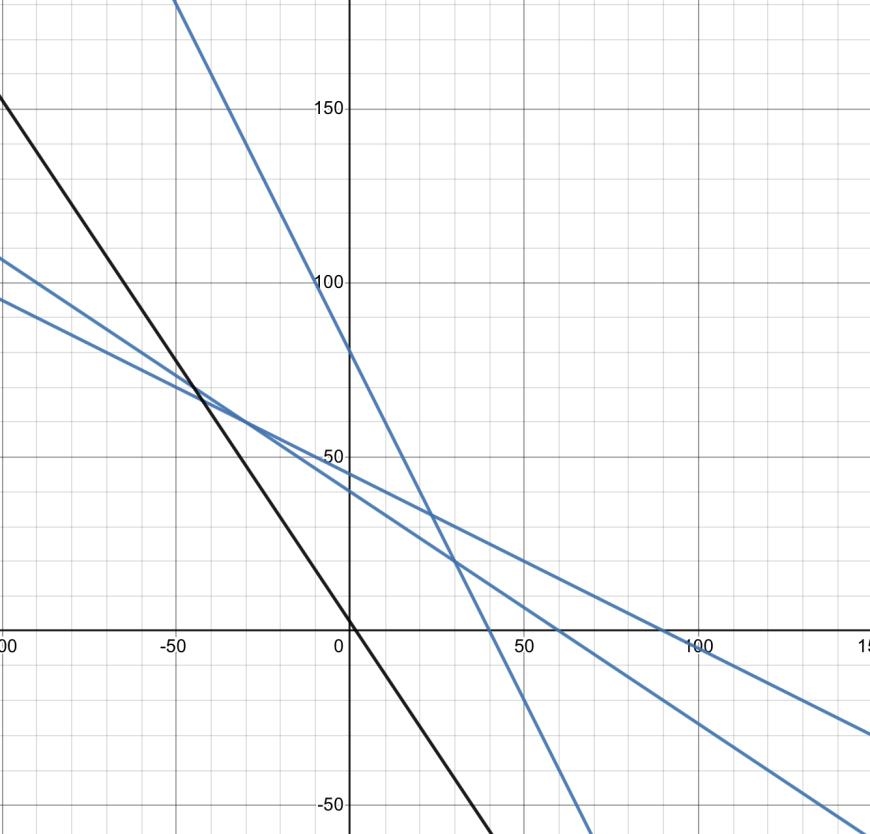
\includegraphics[width = 5cm, right]{images/IMG_keine_Losung.jpeg}
Nichtnegativitätsbedingung:\\
\begin{math}
x_1 >= 0, x_2>= 0\\
\end{math}
Aufgrund der Größer-Gleich-Bedingung muss im Tableau eine künstliche Variable s’3 angelegt werden. Diese muss in den folgenden Iterationen herausgerechnet werden.\\
\begin{table}[!ht]
\begin{tabular}{|l|l|l|l|l|l|l|l|}
\hline
\rowcolor[HTML]{C0C0C0} 
Zeile                      & $x_1$                          & $x_2$                          & $s_1$                        & $s_2$                        & $s_3$                        & s`3 & RS  \\ \hline
\cellcolor[HTML]{C0C0C0}1  & \cellcolor[HTML]{FFFFFF}1/3 & \cellcolor[HTML]{CBCEFB}1/2 & \cellcolor[HTML]{FFFFFF}1 & \cellcolor[HTML]{FFFFFF}0 & \cellcolor[HTML]{FFFFFF}0 & 0   & 20  \\ \hline
\cellcolor[HTML]{C0C0C0}2  & \cellcolor[HTML]{FFFFFF}2   & \cellcolor[HTML]{FFFFFF}1   & \cellcolor[HTML]{FFFFFF}0 & \cellcolor[HTML]{FFFFFF}1 & \cellcolor[HTML]{FFFFFF}0 & 0   & 80  \\ \hline
\cellcolor[HTML]{C0C0C0}3  & \cellcolor[HTML]{FFFFFF}1   & \cellcolor[HTML]{FFFFFF}2   & \cellcolor[HTML]{FFFFFF}0 & \cellcolor[HTML]{FFFFFF}0 & \cellcolor[HTML]{FFFFFF}1 & -1  & 90  \\ \hline
\cellcolor[HTML]{C0C0C0}Z  & \cellcolor[HTML]{FFFFFF}-6  & \cellcolor[HTML]{FFFFFF}-4  & \cellcolor[HTML]{FFFFFF}0 & \cellcolor[HTML]{FFFFFF}0 & \cellcolor[HTML]{FFFFFF}0 & 0   & 0   \\ \hline
\cellcolor[HTML]{C0C0C0}Z2 & -1                          & -2                          & 0                         & 0                         & 0                         & 1   & -90 \\ \hline
\end{tabular}
\end{table}
\\
\begin{table}[!ht]
\begin{tabular}{|l|l|l|l|l|l|l|l|l|}
\hline
\rowcolor[HTML]{C0C0C0} 
Zeile                      & $x_1$                            & $x_2$                        & $s_1$                           & $s_2$                        & $s_3$                        & s`3 & RS  & Rechnung                  \\ \hline
\cellcolor[HTML]{C0C0C0}1  & \cellcolor[HTML]{FFFFFF}2/3   & \cellcolor[HTML]{FFFFFF}1 & \cellcolor[HTML]{FFFFFF}1/2  & \cellcolor[HTML]{FFFFFF}0 & \cellcolor[HTML]{FFFFFF}0 & 0   & 40  & (wurde durch 1/2 geteilt) \\ \hline
\cellcolor[HTML]{C0C0C0}2  & \cellcolor[HTML]{FFFFFF}4/3   & \cellcolor[HTML]{FFFFFF}0 & \cellcolor[HTML]{FFFFFF}-1/2 & \cellcolor[HTML]{FFFFFF}1 & \cellcolor[HTML]{FFFFFF}0 & 0   & 40  & -(Zeile 1)                \\ \hline
\cellcolor[HTML]{C0C0C0}3  & \cellcolor[HTML]{FFFFFF}-1/3  & \cellcolor[HTML]{FFFFFF}0 & \cellcolor[HTML]{FFFFFF}-1   & \cellcolor[HTML]{FFFFFF}0 & \cellcolor[HTML]{FFFFFF}1 & -1  & 10  & -2*(Zeile 1)              \\ \hline
\cellcolor[HTML]{C0C0C0}Z  & \cellcolor[HTML]{FFFFFF}-10/3 & \cellcolor[HTML]{FFFFFF}0 & \cellcolor[HTML]{FFFFFF}2    & \cellcolor[HTML]{FFFFFF}0 & \cellcolor[HTML]{FFFFFF}0 & 0   & 160 & +4*(Zeile 1)              \\ \hline
\cellcolor[HTML]{C0C0C0}Z2 & 1/3                           & 0                         & 1                            & 0                         & 0                         & 1   & -10 & +2*(Zeile 1)              \\ \hline
\end{tabular}
\end{table}
\\
Die künstliche Variable lässt sich nicht herausrechnen, da in der Z2 Zeile keine negativen Werte mehr vorhanden sind. Die Zeile Z2 und die Zeile 3 schließen sich gegenseitig aus, wodurch kein Bereich gefunden werden kann, in dem ein valides Optimum existiert. Es gibt für dieses Optimierungsproblem also keine zulässige Lösung.\\\\\\
\textbf{Degenerierte Lösung: }\\
In diesem Fall existieren mehrere optimale Lösungen, da eine oder mehrere Basisvariablen bereits von Beginn an Null sind. Dadurch kommt es zu keiner Veränderung der rechten Seite des Tableaus, wenn ein Iterationsschritt ausgeführt wird.\\\\
\textbf{Beispiel: }\\
Zielfunktion: max Z = 2*$x_1$+2*$x_2$\\
\\
Nebenbedingungen:\\
\begin{math}
2*x_1 <= 60\\
4*x_1-4*x_2 <= 0\\
\end{math}
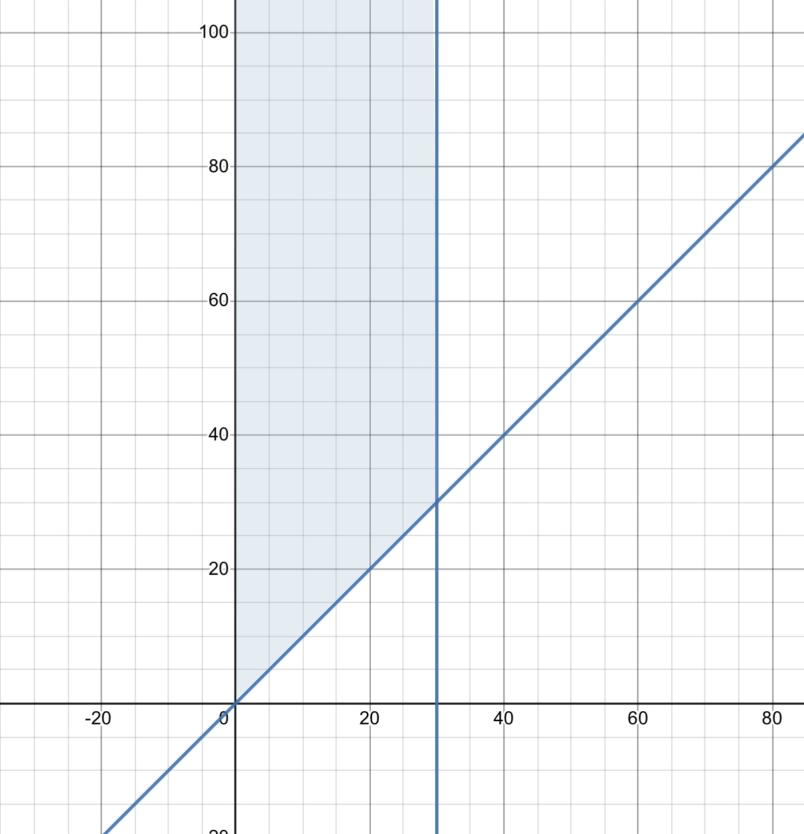
\includegraphics[width=5cm,right]{images/IMG_degenerierte_Losung.jpeg}
Nichtnegativitätsbedingung:\\
\begin{math}
x_1 >= 0, x_2 >= 0
\end{math}
\\
\begin{table}[!ht]
\begin{tabular}{|l|l|l|l|l|l|}
\hline
\rowcolor[HTML]{C0C0C0} 
Zeile                     & $x_1$                       & $x_2$ & $s_1$ & $s_2$ & RS \\ \hline
\rowcolor[HTML]{FFFFFF} 
\cellcolor[HTML]{C0C0C0}1 & 2                         & 0  & 1  & 0  & 60 \\ \hline
\rowcolor[HTML]{FFFFFF} 
\cellcolor[HTML]{C0C0C0}2 & \cellcolor[HTML]{CBCEFB}4 & -4 & 0  & 1  & 0  \\ \hline
\rowcolor[HTML]{FFFFFF} 
\cellcolor[HTML]{C0C0C0}Z & -2                        & -2 & 0  & 0  & 0  \\ \hline
\end{tabular}
\end{table}
\\
\begin{table}[!ht]
\begin{tabular}{|
>{\columncolor[HTML]{C0C0C0}}l |
>{\columncolor[HTML]{FFFFFF}}l |
>{\columncolor[HTML]{FFFFFF}}l |
>{\columncolor[HTML]{FFFFFF}}l |
>{\columncolor[HTML]{FFFFFF}}l |
>{\columncolor[HTML]{FFFFFF}}l |l|}
\hline
Zeile & \cellcolor[HTML]{C0C0C0}$x_1$ & \cellcolor[HTML]{C0C0C0}$x_2$ & \cellcolor[HTML]{C0C0C0}$s_1$ & \cellcolor[HTML]{C0C0C0}$s_2$ & \cellcolor[HTML]{C0C0C0}RS & \cellcolor[HTML]{C0C0C0}Rechnung \\ \hline
1     & 0                          & 2                          & 1                          & -1/2                       & 60                         & -2*(Zeile 2)                     \\ \hline
2     & 1                          & -1                         & 0                          & 1/4                        & 0                          & (wurde durch 4 geteilt)          \\ \hline
Z     & 0                          & -4                         & 0                          & 1/2                        & 0                          & +2*(Zeile 2)                     \\ \hline
\end{tabular}
\end{table}\\
Wie in diesem Beispiel deutlich wird, verändert sich die rechte Seite nicht. Somit gibt es für dieses Problem mehrere optimale Lösungen.







